% Generated by thesis/ch7/exp2/networks.py -- do not edit by hand.
\begin{sidewaysfigure}
  \centering
  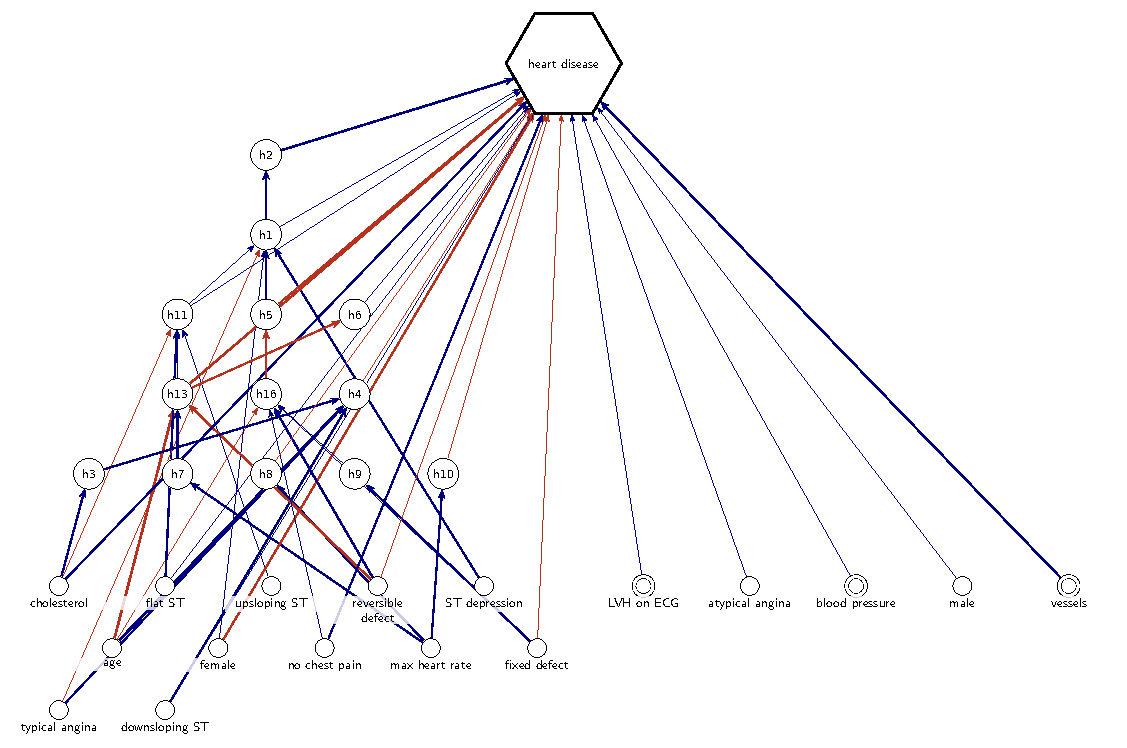
\includegraphics[width=\textheight,height=0.78\textwidth,keepaspectratio]{figures/exp2/networks/heart100-s2-raw}
  \caption{Heart-100, seed 2 (heart100-s2): the network as trained, before any explanation, in full. Inputs at the bottom (every input column its own node), hidden units by depth, the output at the top; 17 of 26 input columns are connected, with 13 hidden units and 50 enabled connections. Blue: positive weight (raises the score); red: negative weight (lowers it); thicker: larger weight. Orange outline and up arrow: raises the final prediction; teal and down arrow: lowers it; grey and double arrow: depends. Not used (no connection; 9 columns): non-anginal pain, sugar 120 or less, sugar above 120, normal ECG, ST-T abnormal ECG, no exercise pain, exercise pain, normal thallium and thallium code 4.}
  \label{fig:exp2-net-heart100-s2-raw}
\end{sidewaysfigure}
